\documentclass[11pt,onecolumn]{IEEEtran}

% For a two-column document, use the following.

% \documentclass[11pt]{IEEEtran}

% For a conference mode document, use the following and see other conference
% mode changes below.

% \documentclass[11pt,conference]{IEEEtran}

\usepackage{graphicx}

% For a fancy header, use the following and see other fancy header changes
% below.

% \usepackage{url}
% \usepackage{fancyhdr}
% \pagestyle{fancy}
% \lhead{}
% \chead{}
% \rhead{\small \sc This is a draft -- for updates please see: \normalfont \url{http://faculty.cs.byu.edu/~zappala}}
% \lfoot{\small 8 February 2005}
% \cfoot{}
% \rfoot{\thepage}
% \renewcommand{\headrulewidth}{0.4pt}

\begin{document}

\title{The Title of a Fantastic Paper}

% For regular mode use this author string:

\author{Emma Bright and Adam Wise\\
\it Computer Science Department\\
Brigham Young University\\
Provo, UT 84602-6576\\
\{bright, wise\}@cs.byu.edu
}

% For conference mode use this author string:

%\author{
%	\authorblockN{Emma Bright and Adam Wise}
%	\authorblockA{\it Computer Science Department\\ 
%			Brigham Young University\\
%			Provo, Utah 84602-6576\\
%			\{bright, wise\}@cs.byu.edu}
%}

\maketitle

% For fancy headers, use the following:

% \thispagestyle{fancy}

% The following sections show examples of what should be included in
% each part of a paper.  If your paper gets to be too long, or if you
% want to collaborate with other writers, it is often helpful to split
% the latex file into multiple files.  You can include a file called
% ``introduction.tex'' by using:
%
% \input introduction

\begin{abstract}

  Describe the problem and your contributions in one short paragraph.
  Include only the most important and relevant items.  Most reports
  for a class project do not need an abstract.

\end{abstract}

\section{Introduction}

Your introduction should focus on clearly describing the problem you
are trying to solve, briefly explain how your solution solves this
problem, and summarize your contributions or results.

Whether you are writing a scientific paper, a proposal, or a report on
a class project, you are usually trying to solve a problem.  It could
be that you are trying to develop an efficient method of peer-to-peer
file transfer or building a scalable web server.  Explain what the
problem is and why it is important.  If this is a scientific paper or
aproposal, you should referene the most significant related work and
explain why this work is not adequate.

Next you should explain your proposed solution and why you think it
solves the problem.  If you are building a scalable web server, for
example, explain your architecture and how it should help the
web server to handle a higher request load.

The final part of the introduction depends on the type of paper you
are writing.  For a scientific paper, you should summarize your
contributions or results.  For a proposal, you should summarize
your proposed area of research and the experiments you will conduct.
For a report on a class project, summarize the status of your project
and what it can do.

\section{Related Work}

For a scientific paper or proposal, you should discuss significant related
work in more detail, relating it to your research question.  This section
may come immediately after the introduction if the treatment of related
work gives necessary background to the body of your paper.  For example,
if you are extending someone else's work, it is a good idea to explain
their work before you discuss your extensions.  In other cases, this section
can come just before the conclusion of your paper, if the work is more
peripheral to what you have done.

In your paper you will likely need to refer to other work.  The best
way to do this is to build a bibliographic database and then reference
those works.  This paper uses the file ``paper.bib'', from which I can
reference an important paper on the design philosophy of the Internet
protocols \cite{internetdesign}, the IETF audiocast using multicast
\cite{mbone}, and even interesting web sites \cite{slashdot}.  LaTeX
will automatically number the references for you and include only
those papers you actually cite.  Please do not use a reference as a
noun when writing a paper, as in ``[12] does some important work''.
Instead, use the following form: ``some important work [12]''.

\section{Body}

The organization of the body of your paper depend on the type of paper
you are writing.  For a scientific paper, you will likely have a
section describing your solution, a section on the methodology you
used to demonstrate the effectiveness of your solution, and then one
or more sections of results.  For a proposal, you will likely have one
section for each major portion of the proposed work.  For a report on
a class project, you may have a section on the overall architecture and
others on each component.

One of the strengths of latex is its handling of mathematical equations.
If you need to include some math in your paper, you have several options.
First, you can include math inline, such as $f(x) = 2x + 5$.  Second,
you can include a list of equations:

\[ f(x) = 2x + 5 \]
\[ g(x) = 4x - 3 \]
therefore
\[ f(x) + g(x) = 6x + 2. \]

If you prefer to number the equations so that you can refer to them
later, you can do that too:

\begin{equation}
f(x) = 2x + 5
\end{equation}

\begin{equation}
g(x) = 4x - 3
\end{equation}

therefore
\begin{equation}
f(x) + g(x) = 6x + 2.
\label{final}
\end{equation}

These equations will be automatically numbered by LaTeX.  If you wish
to refer to an equation, don't explicitly list the number, since the
numbering may change as you revise the paper.  Instead, label the
equations and then you can refer to them with the label.  For example,
Equation~\ref{final} is particularly clever.

You may need to include bulleted lists in your paper, consisting of a
\begin{itemize}
\item first item,
\item second item,
\item third item, and
\item fourth item.
\end{itemize}
If you want to use an enumerated list instead, you can do that too:
\begin{enumerate}
\item First, do the first thing.
\item Second, do the second thing.
\item Third, do the third thing.
\end{enumerate}
These environments can be nested.

In the body of the proposal, you may need to include tables or figures
to explain your results.  Here is an example of a table, cited as
Table~\ref{items}.  Note that I am including some rather complicated
formatting -- a heading that spans multiple columns and some math
inside the table.

\begin{table}
\centering
\begin{tabular}{l | c | c}
\hline
& \multicolumn{2}{| c}{\bf Price} \\ 
{\bf Item for Class} & Dollars & Qoodles ($\sqrt{dollars}$)  \\ \hline \hline
Computer & \$1000 & \$31.62 \\
Goggles & \$7 & \$2.65 \\
Fire Extinguisher & \$20 & \$4.47 \\
\end{tabular}
\caption{Required Items}
\label{items}
\end{table}

When including figures in your paper, one choice you will have to make
is whether to use the PNG or EPS format.  If you process the LaTeX with
the ``latex-dvips-ps2pdf'' sequence, then you need to use EPS format.
If you instead process the LaTeX with ``pdflatex'' then you need to
use the PNG format.  Either way, you can include figures with the
same syntax, shown below.

Figure~\ref{apache} shows you an example of including a figure from a
vector drawing program.  I recommend {\em inkscape} for this purpose
since it uses the SVG format, which is readable by many other programs
for conversion.  {\em inkscape} does a good job of exporting to the
PNG format, though you should be sure to use a white background (the
default is transparent).  It does not export to EPS very well; instead
you can use Gimp to convert the PNG to eps.

\begin{figure}
\centering
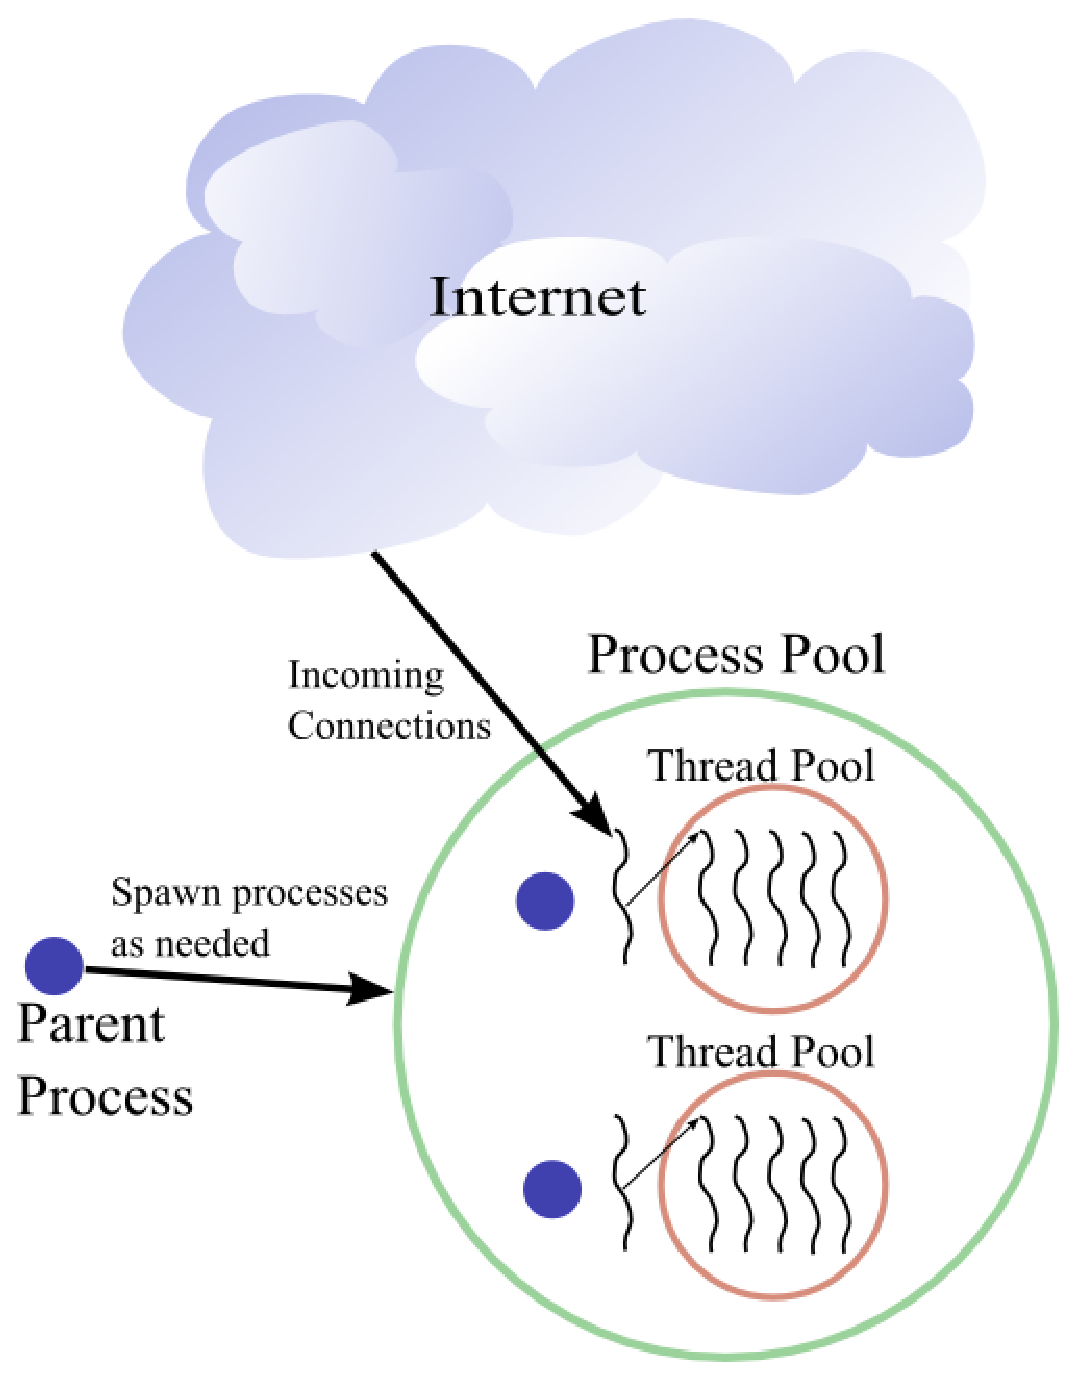
\includegraphics[height=5cm]{apache-thread-mpm}
\caption{Apache Thread Multiprocessing Module}
\label{apache}
\end{figure}

Figure~\ref{tcp} shows you an example of including a figure from a
plotting package.  This example uses a Python script and the biggles
plotting package; I like it because the graphs look clean and it can
export into PNG, EPS, and several other formats.  An alternative is to
use gnuplot.

\begin{figure}
\centering
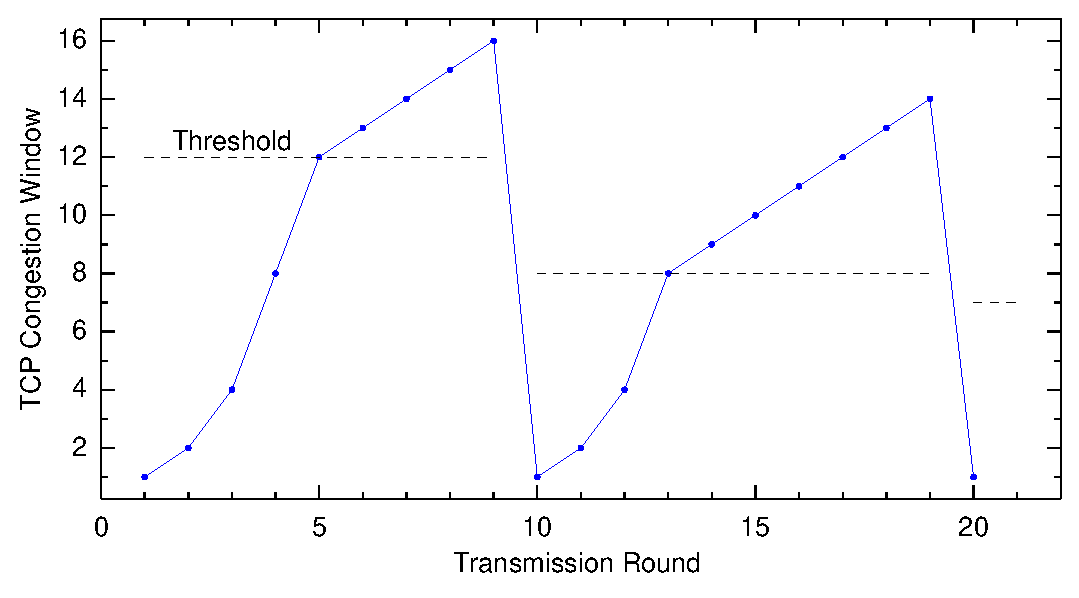
\includegraphics[height=5cm]{tcp}
\caption{TCP Congestion Window}
\label{tcp}
\end{figure}

\section{Conclusions and Future Work}

You should discuss the conclusions that follow from your results.
For example, if you have tested several different ways of building
a scalable web server, you might conclude that one particular architecture
is best.  You should explain how you arrived at this conclusion based
on your results.  You should also suggest areas for future work that
follow naturally from your project.  Explain what you would do if you
had another year to work on the project.

% The following lines show how to include a bibtex-style bibliography,
% formatted according to a particular style.

\bibliographystyle{IEEEtran}
\bibliography{paper}

\appendix

\begin{center}
Appendix Title
\end{center}

If you need to include an appendix, this is how you can do it.

\end{document}
